
\subsection{Vista de implementación}

Se describe la estructura del modelo de implementación, que está totalmente 
relacionado con la herramienta de programación que se utilice para realizar 
la aplicación. En Python las clases de agrupan en paquetes (\textit{package}).

SWAML se ha dividido en dos paquetes, \texttt{swaml} y \texttt{swaml.classes},
tal y como se puede ver en el diagrama de componentes de la 
figura~\ref{fig:uml:implementación}.

\begin{figure}[H]
	\centering
	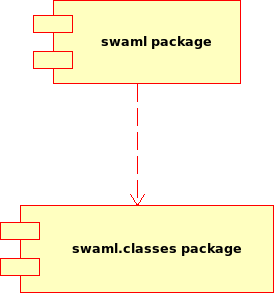
\includegraphics[width=6cm]{images/uml/implementacion.png}
	\caption{Diagrama de implementación}
	\label{fig:uml:implementación}
\end{figure}

En la documentación en linea\footnote{\url{http://swaml.berlios.de/doc/}}
puede obtenerse con más detalle la composición de cada paquete.